\documentclass[11pt]{article}
\usepackage[spanish,es-nodecimaldot,es-tabla]{babel}
% Preambulo comun de los tres documentos (el idioma de babel se carga antes de este archivo)
\usepackage[utf8]{inputenc}
\usepackage[T1]{fontenc}
\usepackage{lmodern}
\usepackage[margin=2.5cm]{geometry}
\usepackage{amsmath,amssymb}
\usepackage{graphicx}
\usepackage{array}
\usepackage{float}
\usepackage{caption}
\usepackage{enumitem}
\usepackage{microtype}
\usepackage[round]{natbib}
\usepackage[hidelinks]{hyperref}
\captionsetup{font=small,labelfont=bf,justification=justified,singlelinecheck=false}
\captionsetup[table]{position=top,skip=6pt}
\renewcommand{\arraystretch}{1.25}
\setlength{\parskip}{0.45em}
\setlength{\parindent}{0pt}
\graphicspath{{figuras/}}
\newcommand{\tabla}[1]{\centering\small\setlength{\tabcolsep}{4.5pt}\input{tablas/#1}}

% Titulos de tablas y figuras (espanol). Compartidos por los documentos y por las versiones PNG.
\newcommand{\capTabA}{Supervivencia de plántulas en LHS-1 según la proporción de sustrato ionitopónico. Los valores se expresan como media $\pm$ desviación estándar (DE); $n = 5$ unidades experimentales por grupo.}
\newcommand{\capTabB}{Análisis de varianza para la proporción de sustrato ionitopónico en LHS-1, particionado en dos contrastes ortogonales planificados.}
\newcommand{\capTabC}{Contrastes planificados para la supervivencia de plántulas en LHS-1. Las diferencias se expresan en puntos porcentuales (pp).}
\newcommand{\capTabD}{Sensibilidad de los contrastes planificados a la elección del término de error y de la unidad de análisis.}
\newcommand{\capTabE}{Contrastes de contexto para la supervivencia de plántulas. Las diferencias se expresan en puntos porcentuales (pp).}
\newcommand{\capTabF}{Análisis de varianza de dos vías para la supervivencia de plántulas según sustrato y tratamiento.}
\newcommand{\capTabG}{Germinación según tratamiento y sustrato. Los valores se expresan como proporciones con intervalos de confianza (IC) exactos (Clopper--Pearson) del 95\,\%.}
\newcommand{\capTabH}{Contrastes seleccionados para la germinación, evaluados a nivel de semilla y a nivel de unidad experimental.}
\newcommand{\capTabI}{Potencia estadística de la fase piloto y tamaño de muestra requerido para un experimento confirmatorio (potencia de 0.80, $\alpha = 0.05$).}
\newcommand{\capFigA}{Supervivencia de plántulas en LHS-1 según la proporción de sustrato ionitopónico. Los puntos representan las medias de grupo y las barras representan $\pm 1$ error estándar (error agrupado, 32 grados de libertad); $n = 5$ unidades experimentales por grupo.}
\newcommand{\capFigB}{Diferencias estimadas en la supervivencia de plántulas con intervalos de confianza bilaterales del 95\,\%. Los marcadores oscuros corresponden a los contrastes planificados de la hipótesis; los marcadores grises corresponden a comparaciones complementarias y de contexto.}
\newcommand{\capFigC}{Supervivencia de plántulas según tratamiento y sustrato. Los puntos representan las medias de grupo y las barras representan $\pm 1$ error estándar (error agrupado, 32 grados de libertad).}
\newcommand{\capFigD}{Germinación según tratamiento y sustrato. Los puntos representan las proporciones observadas y las barras representan intervalos de confianza exactos (Clopper--Pearson) del 95\,\%; 20 semillas por grupo.}
\newcommand{\capFigE}{Potencia estadística para detectar una diferencia de 20 puntos porcentuales en la supervivencia de plántulas en función del número de unidades experimentales por grupo ($\alpha = 0.05$; desviación estándar residual de 31.8 puntos porcentuales). La línea horizontal indica una potencia de 0.80.}
\newcommand{\capFigTA}{Distribución $t$ de Student con 32 grados de libertad bajo la hipótesis nula de C1. El estadístico observado no alcanza la región de rechazo unilateral.}
\newcommand{\capFigTB}{Distribución de permutación exacta de la diferencia de germinación entre el aditivo al 5\,\% y la solución convencional en LHS-1, con la unidad experimental como unidad de análisis (252 reordenamientos de 10 unidades). En azul, los reordenamientos al menos tan extremos como el observado.}

\usepackage{tocloft}
\setlength{\cftsecnumwidth}{2.1em}
\setlength{\cftsubsecnumwidth}{2.9em}
\newcommand{\clave}[1]{\par\smallskip\noindent\fbox{\parbox{0.97\linewidth}{\small\textbf{Idea clave.} #1}}\par\smallskip}
\newcommand{\defensa}[1]{\par\smallskip\noindent\fbox{\parbox{0.97\linewidth}{\small\textbf{Cómo sustentarlo.} #1}}\par\smallskip}

\title{\textbf{Fundamentos matemáticos y estadísticos del análisis}\\[4pt]
\large Documento de estudio: fórmulas, cálculos paso a paso y razones de cada decisión}
\author{}
\date{}

\begin{document}
\maketitle
\vspace{-3em}

\section*{Propósito de este documento}

Este documento acompaña al informe estadístico de la fase piloto. Su objetivo no es presentar resultados nuevos, sino explicar \emph{de dónde sale cada número} y \emph{por qué se tomó cada decisión}, de modo que el análisis pueda defenderse ante un revisor. Cada sección sigue el mismo orden: la idea, la fórmula, el cálculo con los datos del experimento y la razón estadística. Los recuadros de \textbf{Idea clave} resumen lo esencial y los de \textbf{Cómo sustentarlo} proponen el argumento para defender la decisión. Todos los cálculos se realizaron en R (versión 4.3.3) y pueden reproducirse con los archivos \texttt{analisis\_preliminar.R} y \texttt{prueba\_hipotesis.R}.

\tableofcontents

\section{Qué datos hay y qué permiten hacer}

\subsection{Estructura del diseño}

El experimento es un factorial $2 \times 4$: dos sustratos (LHS-1 y arena de río) por cuatro tratamientos (control, aditivo al 5\,\%, aditivo al 10\,\% y solución convencional). Del texto del manuscrito se deduce el tamaño de cada grupo:
\[
\frac{160 \text{ semillas}}{40 \text{ unidades}} = 4 \text{ semillas por unidad}, \qquad
\frac{40 \text{ unidades}}{8 \text{ grupos}} = 5 \text{ unidades por grupo}.
\]
Las tablas confirman esta deducción. Con cuatro semillas, el porcentaje de germinación de una unidad solo puede valer 0, 25, 50, 75 o 100. Una media de 95.0 con desviación estándar de 11.2 solo se obtiene con cinco unidades cuyos valores son $(100, 100, 100, 100, 75)$:
\[
\bar{y} = \frac{4(100) + 75}{5} = 95, \qquad
s = \sqrt{\frac{4(100-95)^2 + (75-95)^2}{5-1}} = \sqrt{\frac{100 + 400}{4}} = \sqrt{125} = 11.18 .
\]

\subsection{Por qué bastan la media, la desviación estándar y el tamaño de grupo}

Sea $y_{ijk}$ el porcentaje de supervivencia de la unidad $k$ del sustrato $i$ y tratamiento $j$. El modelo del ANOVA es
\[
y_{ijk} = \mu_{ij} + \varepsilon_{ijk}, \qquad \varepsilon_{ijk} \sim N(0, \sigma^2) \text{ independientes.}
\]
En este modelo, toda la información sobre las medias $\mu_{ij}$ está en las medias muestrales $\bar{y}_{ij}$, y toda la información sobre $\sigma^2$ está en las varianzas muestrales $s_{ij}^2$ (son los \emph{estadísticos suficientes}). Por eso un ANOVA puede calcularse de forma exacta sin los datos crudos, siempre que se conozcan $\bar{y}_{ij}$, $s_{ij}$ y $n$.

\clave{Lo que \emph{no} puede hacerse sin los datos por unidad es verificar los supuestos (normalidad, valores atípicos) ni ajustar modelos que usen los conteos de cada unidad. Esa es la limitación real de trabajar con tablas resumen, y por eso se declara en el informe.}

\section{La unidad experimental: maceta o semilla}

\subsection{La idea}

La \emph{unidad experimental} es la entidad a la que se asigna el tratamiento de forma independiente. Aquí el tratamiento se aplicó a cada unidad (maceta), no a cada semilla. Las cuatro semillas de una unidad comparten sustrato, riego, posición y luz; por tanto, tienden a parecerse entre sí. Tratar las 160 semillas como 160 observaciones independientes se conoce como \emph{pseudorreplicación} \citep{hurlbert} y hace que la evidencia parezca más fuerte de lo que es.

\subsection{Cómo se mide: la sobredispersión}

Si las semillas de una unidad fueran independientes, el número de sobrevivientes entre $m$ germinadas seguiría una distribución binomial, y la varianza del porcentaje por unidad sería
\[
\operatorname{Var}_{\text{bin}} = 100^2 \, \frac{p(1-p)}{m}.
\]
El cociente entre la varianza observada y la binomial es el factor de sobredispersión $\phi$. Para LHS-1 sin enmendar ($p = 0.55$, $m = 4$, $s = 32.4$):
\[
\operatorname{Var}_{\text{bin}} = 100^2 \, \frac{0.55 \times 0.45}{4} = 618.75, \qquad
\phi = \frac{32.4^2}{618.75} = \frac{1049.76}{618.75} = 1.70 .
\]
Para los grupos con 5\,\% y 10\,\% se obtiene $\phi = 1.54$ y $\phi = 1.43$; el promedio es $\phi = 1.56$.

El factor $\phi$ se relaciona con la correlación intraclase $\rho$ (qué tanto se parecen las semillas de una misma unidad) mediante el \emph{efecto de diseño}:
\[
\phi = 1 + (m - 1)\rho \quad\Longrightarrow\quad \rho = \frac{\phi - 1}{m - 1} = \frac{1.56 - 1}{4 - 1} \approx 0.19 .
\]
Una consecuencia práctica es el \emph{tamaño de muestra efectivo}: $N_{\text{ef}} = N / \phi$. Las 20 semillas de un grupo equivalen, en información, a unas $20/1.56 \approx 13$ semillas independientes.

\clave{Las propias tablas muestran que las unidades varían 1.56 veces más de lo esperado si las semillas fueran independientes. Por eso todo el análisis principal toma la unidad experimental como unidad de análisis.}

\defensa{``El tratamiento se asignó a la unidad experimental, no a la semilla. Además, la varianza entre unidades fue 1.56 veces la binomial, lo que confirma que las semillas de una misma unidad no son independientes. Analizar por semilla inflaría la evidencia.''}

\section{ANOVA a partir de estadísticos resumen}

\subsection{Fórmulas}

Para un factorial balanceado con $a$ sustratos, $b$ tratamientos y $n$ unidades por grupo, las sumas de cuadrados (SC) son
\begin{align*}
\text{SC}_A &= b\,n \sum_{i=1}^{a} (\bar{y}_{i\cdot} - \bar{y}_{\cdot\cdot})^2, &
\text{SC}_B &= a\,n \sum_{j=1}^{b} (\bar{y}_{\cdot j} - \bar{y}_{\cdot\cdot})^2, \\
\text{SC}_{\text{grupos}} &= n \sum_{i,j} (\bar{y}_{ij} - \bar{y}_{\cdot\cdot})^2, &
\text{SC}_{AB} &= \text{SC}_{\text{grupos}} - \text{SC}_A - \text{SC}_B ,
\end{align*}
y el cuadrado medio del error (CME), que estima $\sigma^2$, es el promedio de las varianzas de los grupos:
\[
\text{CME} = \frac{1}{ab} \sum_{i,j} s_{ij}^2, \qquad \text{gl}_{\text{error}} = ab(n-1).
\]
Cada efecto se prueba con $F = \text{CM}_{\text{efecto}} / \text{CME}$, que bajo la hipótesis nula sigue una distribución $F$ con los grados de libertad del efecto y del error.

\subsection{Cálculo con los datos de supervivencia}

Las ocho desviaciones estándar son 32.4, 29.6, 22.4, 37.3 (LHS-1) y 20.4, 37.1, 39.1, 31.2 (arena de río). Entonces
\[
\text{CME} = \frac{32.4^2 + 29.6^2 + 22.4^2 + 37.3^2 + 20.4^2 + 37.1^2 + 39.1^2 + 31.2^2}{8} = \frac{8113.79}{8} = 1014.2,
\]
con $8 \times (5 - 1) = 32$ grados de libertad. Su raíz, $\sqrt{1014.2} = 31.8$ puntos porcentuales, es la desviación estándar residual: lo que típicamente se aparta una unidad de la media de su grupo.

Las medias de los sustratos son 67.075 (LHS-1) y 51.65 (arena de río), y la media general es 59.3625. Para el sustrato:
\[
\text{SC}_A = 4 \times 5 \times \left[(67.075 - 59.3625)^2 + (51.65 - 59.3625)^2\right] = 20 \times 2 \times 59.48 = 2379.3,
\]
\[
F = \frac{2379.3 / 1}{1014.2} = 2.35, \qquad p = P(F_{1,32} \ge 2.35) = 0.135 .
\]
La Tabla~\ref{tab:anova-factorial} presenta el análisis completo.

\begin{table}[H]
\caption{\capTabF}\label{tab:anova-factorial}
\tabla{tabF_anova_factorial_es}
\end{table}

El $\eta^2$ parcial, $\text{SC}_{\text{efecto}} / (\text{SC}_{\text{efecto}} + \text{SC}_{\text{error}})$, indica qué fracción de la variación no explicada por los demás efectos se atribuye a ese efecto. Para el sustrato, $2379.3 / (2379.3 + 32455.2) = 0.068$.

\subsection{Supuestos y qué tan razonables son aquí}

\begin{itemize}[leftmargin=1.4em,itemsep=2pt]
\item \textbf{Independencia entre unidades.} Es razonable si cada unidad se manejó por separado. La cercanía física entre unidades de una misma ubicación podría introducir alguna dependencia (ver Sección~\ref{sec:luz}).
\item \textbf{Varianzas iguales.} La razón entre la varianza mayor y la menor es $39.1^2 / 20.4^2 = 3.67$. En diseños balanceados, la prueba $F$ tolera razones de este orden; como respaldo se calculó además la versión de Welch, que no supone varianzas iguales (Sección~\ref{sec:error}).
\item \textbf{Normalidad.} No puede verificarse sin los datos por unidad. Con cuatro semillas, el porcentaje de cada unidad toma muy pocos valores, por lo que la normalidad es solo aproximada. Esta es una limitación declarada.
\end{itemize}

\subsection{Por qué el ANOVA no es adecuado para la germinación}

Tres de los ocho grupos tienen germinación de $100.0 \pm 0.0$: su varianza es cero. Las varianzas de los grupos van de 0 a $41.8^2 = 1747$, de modo que el supuesto de varianzas iguales se viola por completo, y la respuesta choca con el techo de 100\,\%. Si aun así se calcula el ANOVA sobre porcentajes, el tratamiento da $p = 0.070$ y la interacción $p = 0.055$; estos valores no son confiables porque se apoyan en un error promedio que no representa a ningún grupo. Por eso la germinación se trató como respuesta binomial (Sección~\ref{sec:germinacion}).

\defensa{``El ANOVA es apropiado para la supervivencia porque sus varianzas son comparables entre grupos. No lo es para la germinación porque tres grupos no tienen variabilidad y la respuesta está acotada en 100\,\%; ahí corresponde un análisis binomial.''}

\section{Contrastes lineales: cómo se traduce una hipótesis en una prueba}

\subsection{Definición y fórmulas}

Un \emph{contraste} es una combinación lineal de medias cuyos coeficientes suman cero:
\[
L = \sum_i c_i \mu_i, \qquad \sum_i c_i = 0 .
\]
Su estimador, su error estándar (EE) y su estadístico de prueba son
\[
\hat{L} = \sum_i c_i \bar{y}_i, \qquad
\text{EE}(\hat{L}) = \sqrt{\text{CME} \, \frac{\sum_i c_i^2}{n}}, \qquad
t = \frac{\hat{L}}{\text{EE}(\hat{L})} \sim t_{\nu} \ \text{ bajo } H_0,
\]
donde $\nu$ son los grados de libertad del error. El intervalo de confianza del 95\,\% es $\hat{L} \pm t_{0.975,\nu}\,\text{EE}(\hat{L})$. Cada contraste tiene además una suma de cuadrados con un grado de libertad:
\[
\text{SC}_L = \frac{n\,\hat{L}^2}{\sum_i c_i^2}, \qquad F = \frac{\text{SC}_L}{\text{CME}} = t^2 .
\]

\subsection{Los dos contrastes de la hipótesis}

La hipótesis del manuscrito tiene dos afirmaciones sobre la supervivencia en LHS-1: (1) el simulante enmendado supera al no enmendado, y (2) la respuesta depende de la proporción. Con las medias $(\bar{y}_0, \bar{y}_5, \bar{y}_{10}) = (55, 65, 85)$:

\textbf{C1, enmendado frente a sin enmendar.} Coeficientes $(-1, \tfrac12, \tfrac12)$:
\[
\hat{L}_1 = -55 + \tfrac12(65) + \tfrac12(85) = 20.0, \qquad
\text{EE} = \sqrt{1014.2 \times \frac{1 + 0.25 + 0.25}{5}} = \sqrt{304.27} = 17.44,
\]
\[
t = \frac{20.0}{17.44} = 1.147, \qquad \text{IC 95\,\%: } 20.0 \pm 2.037 \times 17.44 = [-15.5,\ 55.5].
\]

\textbf{C2, 10\,\% frente a 5\,\%.} Coeficientes $(0, -1, 1)$:
\[
\hat{L}_2 = 85 - 65 = 20.0, \qquad
\text{EE} = \sqrt{1014.2 \times \frac{2}{5}} = 20.14, \qquad
t = 0.993, \qquad \text{IC 95\,\%: } [-21.0,\ 61.0].
\]

\subsection{Ortogonalidad: por qué estos dos contrastes ``reparten'' el ANOVA}

Dos contrastes son \emph{ortogonales} si $\sum_i c_i d_i = 0$. Aquí, $(-1)(0) + (\tfrac12)(-1) + (\tfrac12)(1) = 0$. Cuando los contrastes son ortogonales responden preguntas que no se solapan, y sus sumas de cuadrados suman exactamente la variación entre grupos:
\[
\text{SC}_{C1} = \frac{5 \times 20^2}{1.5} = 1333.3, \qquad
\text{SC}_{C2} = \frac{5 \times 20^2}{2} = 1000.0, \qquad
1333.3 + 1000.0 = 2333.3 = \text{SC}_{\text{dosis}} .
\]
Esto es lo que muestra la Tabla~\ref{tab:anova-dose}: el ANOVA de una vía de la dosis (2 grados de libertad) dividido en dos preguntas de 1 grado de libertad cada una. Se verifica también que $t^2 = F$: $1.147^2 = 1.31$ y $0.993^2 = 0.99$.

\begin{table}[H]
\caption{\capTabB}\label{tab:anova-dose}
\tabla{tabB_anova_dosis_es}
\end{table}

\clave{La prueba $F$ global de la dosis ($p = 0.329$) pregunta ``¿hay \emph{alguna} diferencia entre las tres medias?''. Los contrastes planificados preguntan exactamente lo que dice la hipótesis. Concentrar la prueba en un grado de libertad le da más potencia que la prueba global, y la conclusión se lee directamente en términos de la hipótesis.}

\subsection{Prueba unilateral y bilateral}\label{sec:unilateral}

En una prueba \emph{bilateral} se rechaza $H_0$ si la diferencia es grande en cualquiera de los dos sentidos; el valor $p$ es el área de las dos colas. En una prueba \emph{unilateral} se rechaza solo si la diferencia va en el sentido que predice la hipótesis; el valor $p$ es el área de una cola. Para C1:
\[
p_{\text{unilateral}} = P(t_{32} \ge 1.147) = 0.130, \qquad
p_{\text{bilateral}} = 2 \times 0.130 = 0.260 .
\]
El valor crítico también cambia: 1.694 para la prueba unilateral frente a 2.037 para la bilateral (Figura~\ref{fig:t}).

\begin{figure}[H]
\centering
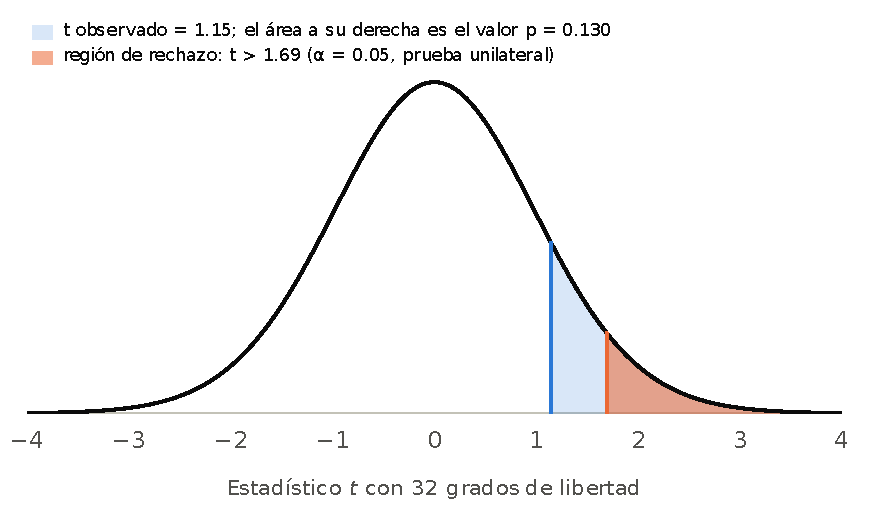
\includegraphics[width=0.8\linewidth]{figT1_distribucion_t_es}
\caption{\capFigTA}\label{fig:t}
\end{figure}

La prueba unilateral es legítima únicamente cuando la dirección del efecto se estableció \emph{antes} de ver los resultados. La razón es sencilla: si primero se observa hacia dónde van los datos y después se elige la cola, la probabilidad real de un falso positivo deja de ser 5\,\% y pasa a ser 10\,\%. Esta era la pregunta que quedó pendiente: \emph{¿la frase de la hipótesis (``higher survival'') se escribió antes de conocer los resultados?} Si la respuesta es sí, C1 se reporta como unilateral con tranquilidad. Si no hay certeza, lo prudente es reportar el valor bilateral. En este caso la decisión no cambia la conclusión, porque ninguno de los dos valores es menor que 0.05; por eso el informe presenta ambos.

C2 se probó de forma bilateral porque la hipótesis dice que la respuesta ``variará'' con la proporción, sin indicar en qué sentido.

\subsection{La tendencia lineal}

Para dosis igualmente espaciadas (0, 5, 10), los coeficientes de la tendencia lineal son $(-1, 0, 1)$, que coinciden con la comparación entre 10\,\% y 0\,\%: $\hat{L} = 85 - 55 = 30.0$, $t = 1.49$, $p$ unilateral $= 0.073$. Dividiendo entre la distancia entre dosis se obtiene la pendiente: $30.0 / 10 = 3.0$ puntos porcentuales por cada 1\,\% de sustrato ionitopónico, con IC 95\,\% de $-1.1$ a $7.1$.

\begin{table}[H]
\caption{\capTabC}\label{tab:contrasts}
\tabla{tabC_contrastes_es}
\end{table}

\defensa{``La hipótesis hace dos afirmaciones; cada una se tradujo en un contraste definido antes del análisis. Son ortogonales, de modo que juntos descomponen exactamente la variación entre las tres proporciones. Ninguno alcanzó significancia: $t_{32} = 1.15$ ($p$ unilateral $= 0.130$) y $t_{32} = 0.99$ ($p = 0.328$).''}

\section{Elección del término de error}\label{sec:error}

El EE de un contraste depende de cómo se estime $\sigma^2$. Hay tres opciones razonables:

\begin{enumerate}[leftmargin=1.6em,itemsep=2pt]
\item \textbf{Error agrupado de los ocho grupos} (CME $= 1014.2$, 32 gl). Usa toda la información del experimento. Supone que la variabilidad entre unidades es la misma en todos los grupos.
\item \textbf{Error solo de los grupos del contraste.} Para C1 se promedian las varianzas de los tres grupos de LHS-1: $(32.4^2 + 29.6^2 + 22.4^2)/3 = 809.2$, con 12 gl. Supone varianzas iguales solo entre esos grupos, pero dispone de menos grados de libertad, lo que eleva el valor crítico (1.782 frente a 1.694).
\item \textbf{Welch--Satterthwaite} \citep{welch,satterthwaite}. No supone varianzas iguales:
\[
\text{EE}^2 = \sum_i \frac{c_i^2 s_i^2}{n}, \qquad
\nu = \frac{\left(\sum_i v_i\right)^2}{\sum_i v_i^2/(n-1)}, \quad v_i = \frac{c_i^2 s_i^2}{n}.
\]
Para C1 resulta $\text{EE} = 16.70$ y $\nu = 6.7$.
\end{enumerate}

\begin{table}[H]
\caption{\capTabD}\label{tab:sensitivity}
\tabla{tabD_sensibilidad_es}
\end{table}

Se eligió la primera opción como análisis principal por tres razones: es la convención en diseños factoriales; con solo cinco unidades por grupo, una varianza estimada con 32 gl es mucho más estable que una estimada con 12 o con 7; y la razón de varianzas (3.67) no sugiere una heterogeneidad grave. Las otras dos se reportan como análisis de sensibilidad.

\clave{El término de error se fijó por criterios de diseño, no por su resultado. De hecho, la opción elegida da el valor $p$ menos favorable para C1 (0.130 frente a 0.112), lo cual es un buen argumento de integridad: no se escogió el análisis que más convenía.}

\section{Comparaciones múltiples}

\subsection{El problema}

Si se hacen $m$ pruebas independientes con $\alpha = 0.05$ y todas las hipótesis nulas son ciertas, la probabilidad de obtener al menos un falso positivo es
\[
1 - (1 - \alpha)^m, \qquad \text{por ejemplo } 1 - 0.95^8 = 0.34 \text{ para } m = 8 .
\]
Por eso, cuantas más comparaciones se hagan, más cautela exige cada resultado ``significativo''.

\subsection{El procedimiento de Holm}

El procedimiento de \citet{holm} controla esa probabilidad y es siempre al menos tan potente como Bonferroni. Se ordenan los valores $p$ de menor a mayor, $p_{(1)} \le \dots \le p_{(m)}$, y el valor ajustado es
\[
\tilde{p}_{(i)} = \max_{j \le i} \left\{ \min\!\left[1,\ (m - j + 1)\, p_{(j)}\right] \right\}.
\]
Con los dos contrastes planificados ($m = 2$): el menor, 0.130, se multiplica por 2 y da 0.260; el mayor, 0.328, se multiplica por 1 y queda en 0.328.

\subsection{La prueba de Tukey}

Para comparar todos los pares de tratamientos se usó la prueba de Tukey, basada en la distribución del rango estudentizado $q$. El intervalo simultáneo de cada diferencia es
\[
(\bar{y}_j - \bar{y}_{j'}) \pm \frac{q_{0.95;\,4,\,32}}{\sqrt{2}} \sqrt{\text{CME} \, \frac{2}{2n}} = (\bar{y}_j - \bar{y}_{j'}) \pm 38.6 .
\]
Ninguna diferencia entre tratamientos supera 38.6 puntos (la mayor es 21.7), de modo que ninguna es significativa ($p \ge 0.438$).

\subsection{Qué se ajustó y qué no}

Los dos contrastes planificados forman la familia confirmatoria y se ajustaron con Holm. Las demás comparaciones (de contexto, factoriales y de germinación) son exploratorias: se reportan sin ajuste conjunto y se declaran como tales. Lo importante es la transparencia: el lector sabe qué se planificó y qué se exploró.

\section{La germinación como respuesta binomial}\label{sec:germinacion}

\subsection{De las medias a los conteos}

Con 20 semillas por grupo (5 unidades de 4 semillas), la media de los porcentajes por unidad coincide con el porcentaje global, así que el número de semillas germinadas es $k = 20 \times \bar{y}/100$. Por ejemplo, 65.0\,\% corresponde a 13 de 20.

\subsection{Intervalo exacto de Clopper--Pearson}

El intervalo de \citet{clopper} se construye con cuantiles de la distribución beta y garantiza una cobertura de al menos 95\,\%:
\[
p_{\text{inf}} = B\!\left(\tfrac{\alpha}{2};\ k,\ n - k + 1\right), \qquad
p_{\text{sup}} = B\!\left(1 - \tfrac{\alpha}{2};\ k + 1,\ n - k\right).
\]
Cuando germinan todas las semillas ($k = n = 20$) el límite inferior tiene forma cerrada: $(\alpha/2)^{1/n} = 0.025^{1/20} = 0.832$. Es decir, observar 20 de 20 es compatible con una germinación real tan baja como 83\,\%.

\subsection{Prueba exacta de Fisher}

Para comparar dos proporciones, la prueba exacta de Fisher calcula, con la distribución hipergeométrica, la probabilidad de tablas tan extremas como la observada, dados los totales. Para la solución convencional (31 de 40) frente al control (40 de 40), hay 9 semillas no germinadas entre 80, todas en un mismo grupo:
\[
p = 2 \times \frac{\binom{40}{9}}{\binom{80}{9}} = 2 \times 0.00118 = 0.0024 .
\]

\subsection{Prueba exacta de tendencia}

Para dosis ordenadas se usa el estadístico de Cochran--Armitage \citep{cochran,armitage}, $T = \sum_i d_i x_i$, donde $d_i$ es la dosis y $x_i$ el número de éxitos. La versión exacta enumera todas las tablas posibles con los mismos totales (distribución hipergeométrica multivariada) y suma las probabilidades de aquellas con $T$ al menos tan extremo como el observado.

\subsection{Intervalo de Newcombe para una diferencia de proporciones}

El intervalo de \citet{newcombe} combina los intervalos de Wilson $(l_1, u_1)$ y $(l_2, u_2)$ de cada proporción:
\[
\left[\, (\hat{p}_1 - \hat{p}_2) - \sqrt{(\hat{p}_1 - l_1)^2 + (u_2 - \hat{p}_2)^2},\ \
(\hat{p}_1 - \hat{p}_2) + \sqrt{(u_1 - \hat{p}_1)^2 + (\hat{p}_2 - l_2)^2} \,\right].
\]
Se eligió porque funciona bien con muestras pequeñas y con proporciones de 0 o 100\,\%, donde el intervalo clásico (de Wald) falla.

\subsection{El modelo logístico y el problema de la separación}

El modelo binomial con enlace logit, $\operatorname{logit}(p_{ij}) = \eta_{ij}$, es el equivalente del ANOVA para proporciones. Con grupos al 100\,\% aparece la \emph{separación}: el estimador de $\operatorname{logit}(1)$ es $+\infty$ y los coeficientes no convergen. Sin embargo, la verosimilitud sí converge, y la comparación de modelos por \emph{devianza} sigue siendo válida. El análisis de devianza dio 15.3 con 3 gl para el tratamiento ($p = 0.0015$) y 11.4 con 3 gl para la interacción ($p = 0.0097$). Estos valores suponen semillas independientes.

\subsection{La prueba de permutación con la unidad como unidad de análisis}

La prueba de permutación responde: \emph{si el tratamiento no tuviera efecto, ¿qué tan raro sería ver una diferencia como la observada solo por la forma en que las unidades quedaron repartidas?} Se calculan todas las formas de repartir las unidades entre los grupos y la proporción de repartos que producen una diferencia al menos tan grande como la observada es el valor $p$.

Ejemplo exacto: en LHS-1, las cinco unidades con aditivo al 5\,\% tuvieron $(4, 4, 4, 4, 4)$ semillas germinadas y las cinco con solución convencional $(4, 4, 3, 2, 0)$. Hay $\binom{10}{5} = 252$ formas de repartir las diez unidades en dos grupos de cinco. La diferencia observada (35 puntos) es la más extrema posible y ocurre siempre que las tres unidades ``bajas'' (3, 2 y 0) quedan en el mismo grupo:
\[
p = \frac{2 \times \binom{7}{2}}{\binom{10}{5}} = \frac{2 \times 21}{252} = 0.167 .
\]

\begin{figure}[H]
\centering
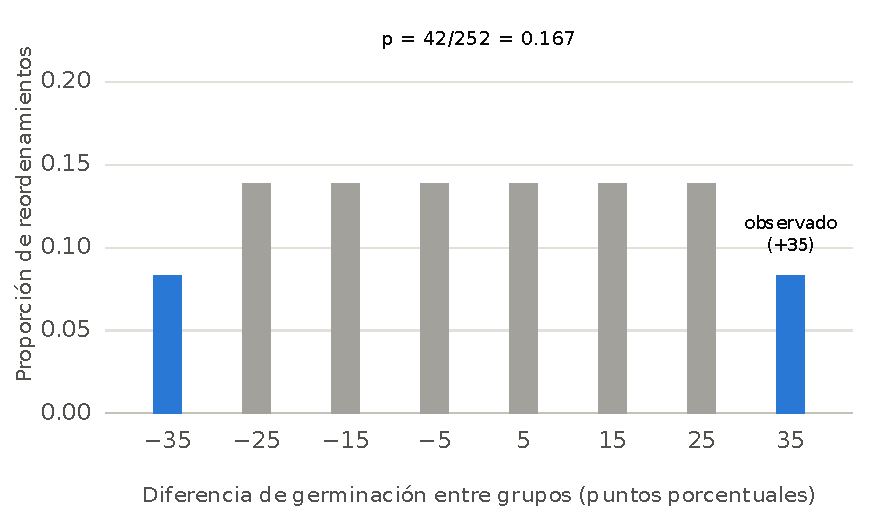
\includegraphics[width=0.8\linewidth]{figT2_permutacion_es}
\caption{\capFigTB}\label{fig:perm}
\end{figure}

\clave{Con cinco unidades por grupo y las semillas no germinadas concentradas en tres unidades, el valor $p$ a nivel de unidad \emph{no puede} ser menor que 0.167, por extrema que sea la diferencia. La prueba de Fisher da $p = 0.008$ para la misma comparación porque cuenta 20 semillas ``independientes'' por grupo. Esa es la diferencia entre los dos niveles de análisis.}

\subsection{Corrección cuasi-binomial}

Una alternativa intermedia es mantener el modelo binomial pero dividir la devianza por el factor de sobredispersión estimado, $\hat\phi = X^2/\text{gl}$ \citep{mccullagh}, y usar una prueba $F$:
\[
F = \frac{\Delta \text{Devianza} / \text{gl}}{\hat\phi}.
\]
Con $\hat\phi$ entre 1.47 y 1.60 (según la configuración de una unidad que no pudo determinarse de forma única), el tratamiento da $F = 15.3/3/1.60 = 3.19$ ($p = 0.046$) o $F = 3.48$ ($p = 0.035$), y la interacción da $p$ entre 0.082 y 0.101.

\subsection{Cómo conciliar los tres resultados}

\begin{center}
\small
\begin{tabular}{lcc}
\hline\hline
\textbf{Análisis del efecto del tratamiento} & \textbf{Supone} & \textbf{$p$} \\
\hline
Fisher exacto a nivel de semilla & Semillas independientes & 0.003 \\
Devianza cuasi-binomial & Sobredispersión constante & 0.035--0.046 \\
Contrastes por permutación a nivel de unidad & Solo la aleatorización de unidades & $\ge 0.065$ \\
\hline
\end{tabular}
\end{center}

A medida que el análisis respeta mejor la estructura real del experimento, la evidencia se debilita. La lectura honesta es que existe una señal (menor germinación con la solución convencional en LHS-1), pero depende de tres unidades y no es robusta.

\defensa{``A nivel de semilla el efecto parece significativo, pero las semillas de una unidad no son independientes. Tomando la unidad como unidad de análisis, ninguna comparación alcanza significancia. Se reportan ambos niveles y se considera el de unidad como evidencia principal.''}

\section{La supervivencia a nivel de semilla}

\subsection{Cómo se recuperan los conteos}

La supervivencia se calculó como el promedio de las razones (sobrevivientes/germinadas) de cada unidad. En LHS-1 con 0\,\% y 5\,\%, todas las unidades tuvieron 4 germinadas, así que la media de razones equivale al cociente global: 55\,\% $\to$ 11 de 20 y 65\,\% $\to$ 13 de 20. Con 10\,\%, las germinadas por unidad fueron $(4, 4, 4, 4, 3)$ y la media de 85\,\% implica que las razones suman $5 \times 0.85 = 4.25$. La unidad con 3 germinadas solo puede aportar 0, $\tfrac13$, $\tfrac23$ o 1; el único valor que deja al resto como múltiplo de $\tfrac14$ y no mayor que 4 es 1. Por tanto las otras cuatro suman $3.25 = 13/4$, y el total es $13 + 3 = 16$ sobrevivientes de 19.

\subsection{La tendencia a nivel de semilla y su corrección}

Con 11/20, 13/20 y 16/19, la prueba exacta de tendencia da $p$ unilateral $= 0.038$ y la versión asintótica $z = 1.95$. Es el único resultado por debajo de 0.05 en todo el análisis de la hipótesis. No se adoptó como resultado principal por dos razones:

\begin{enumerate}[leftmargin=1.6em,itemsep=2pt]
\item Supone semillas independientes, y los datos muestran $\phi = 1.56$. La corrección de tipo \citet{raoscott} divide el estadístico por $\sqrt{\phi}$:
\[
z_{\text{corr}} = \frac{1.95}{\sqrt{1.56}} = 1.56, \qquad p = 0.059,
\]
que coincide con el análisis por unidad ($p = 0.073$).
\item Elegir, entre varios análisis, el único que resulta significativo \emph{después} de ver los resultados invalida el valor $p$. El análisis principal se definió antes y por criterios de diseño.
\end{enumerate}

\defensa{``Se reporta con transparencia que un análisis a nivel de semilla da $p = 0.038$, pero ese análisis ignora el agrupamiento por unidad; al corregirlo, $p = 0.059$. La tendencia es sugerente, no concluyente.''}

\section{La confusión con la luz}\label{sec:luz}

El DLI se midió por ubicación de cultivo, y cada ubicación albergó dos tratamientos de un mismo sustrato:

\begin{center}
\small
\begin{tabular}{clll}
\hline\hline
\textbf{DLI} & \textbf{Sustrato} & \textbf{Tratamientos en esa ubicación} \\
\hline
8.87 & Arena de río & Control y aditivo 5\,\% \\
9.52 & LHS-1 & Aditivo 10\,\% y convencional \\
10.73 & LHS-1 & Control y aditivo 5\,\% \\
10.77 & Arena de río & Aditivo 10\,\% y convencional \\
\hline
\end{tabular}
\end{center}

Cuatro ubicaciones equivalen a 3 grados de libertad, que coinciden exactamente con tres efectos del diseño: el sustrato, el par de tratamientos (control y 5\,\% frente a 10\,\% y convencional) y su interacción. Se dice que esos efectos están \emph{confundidos} (o \emph{aliados}) con la ubicación: cualquier diferencia entre ubicaciones (luz, temperatura, corrientes de aire) es indistinguible de ellos.

Las únicas comparaciones libres de esta confusión son las que se hacen \emph{dentro} de una misma ubicación: 5\,\% frente al control, y 10\,\% frente a la solución convencional. Para la hipótesis, esto significa que C2 (10\,\% frente a 5\,\%) y la mitad de C1 comparan grupos de ubicaciones distintas.

El DLI no pudo usarse como covariable porque solo hay cuatro valores distintos y su desviación estándar mide la variación entre días, no entre unidades. La correlación entre las ocho medias de grupo fue $r = -0.02$; su intervalo se obtiene con la transformación $z$ de Fisher, cuyo error estándar es $1/\sqrt{n - 3} = 1/\sqrt{5} = 0.447$:
\[
\tanh\!\left(\operatorname{artanh}(-0.02) \pm 1.96 \times 0.447\right) = [-0.71,\ 0.69].
\]
Un intervalo tan amplio indica que ocho puntos no permiten afirmar ni descartar una relación.

\defensa{``La luz se registró por ubicación y cada ubicación tuvo tratamientos fijos, de modo que luz y tratamiento no pueden separarse. Por eso no se usó como covariable, se declara como limitación y se recomienda aleatorizar las posiciones en la fase confirmatoria.''}

\section{Potencia y tamaño de muestra}

\subsection{La idea y la fórmula}

La \emph{potencia} es la probabilidad de rechazar $H_0$ cuando el efecto real tiene un tamaño $\Delta$. Si el efecto existe, el estadístico $t$ sigue una distribución $t$ \emph{no central} con parámetro
\[
\delta = \frac{\Delta}{\sigma \sqrt{\sum_i c_i^2 / n}}, \qquad
\text{Potencia (unilateral)} = P\!\left(t_{\nu}(\delta) > t_{1-\alpha,\,\nu}\right).
\]

\subsection{Cálculo}

Para C1 con el diseño del piloto ($n = 5$, $\nu = 32$, $\Delta = 20$, $\sigma = 31.8$):
\[
\delta = \frac{20}{31.8 \sqrt{1.5/5}} = 1.15, \qquad \text{Potencia} = P(t_{32}(1.15) > 1.694) = 0.30 .
\]
Es decir, aun si la enmienda realmente aumentara la supervivencia en 20 puntos, un experimento de este tamaño lo detectaría solo 3 de cada 10 veces. Buscando el menor $n$ que alcanza una potencia de 0.80 se obtiene $n = 24$ unidades por grupo para C1 y $n = 41$ para C2 (Tabla~\ref{tab:power}, Figura~\ref{fig:power}).

\begin{table}[H]
\caption{\capTabI}\label{tab:power}
\tabla{tabI_potencia_es}
\end{table}

\begin{figure}[H]
\centering
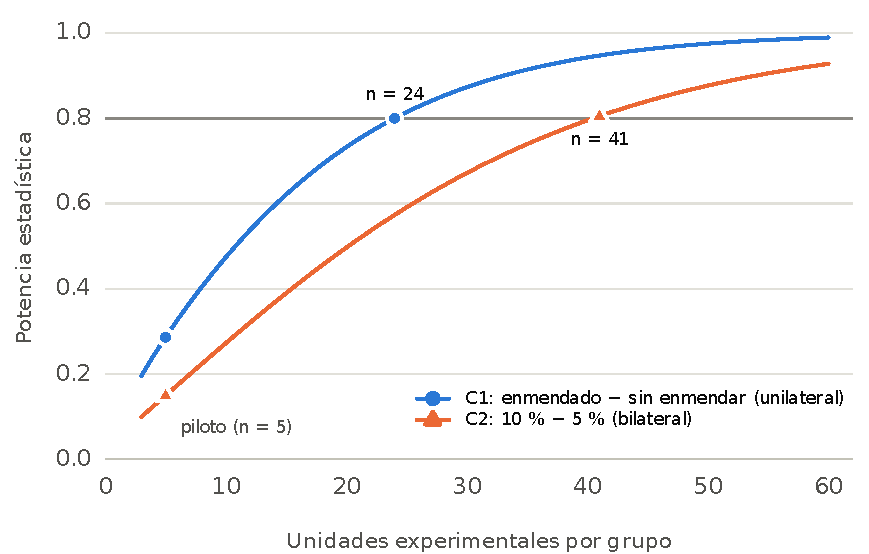
\includegraphics[width=0.75\linewidth]{figE_potencia_es}
\caption{\capFigE}\label{fig:power}
\end{figure}

\subsection{Dos advertencias importantes}

\textbf{La potencia calculada con el efecto observado debe leerse con cautela.} El efecto estimado en un piloto pequeño es muy impreciso (su IC va de $-15.5$ a 55.5), y la potencia ``observada'' es solo otra forma de expresar el valor $p$ \citep{hoenig}. Su utilidad aquí es de planificación. Lo recomendable es fijar, con criterio agronómico, la menor diferencia que tendría importancia práctica y calcular el tamaño de muestra para ese valor.

\textbf{``No significativo'' no significa ``sin efecto''.} El IC de C1 incluye el 0, pero también incluye mejoras de más de 50 puntos. El resultado correcto es ``no concluyente''. Para afirmar que dos tratamientos son equivalentes (por ejemplo, que la enmienda iguala a la solución convencional) se necesita otra prueba: se define un margen $\pm\Delta_0$ y se demuestra que el IC completo cae dentro de él (procedimiento de dos pruebas unilaterales, TOST; \citealp{schuirmann}). Con un IC de $-23.8$ a 47.2, aquí no es posible para ningún margen razonable.

\section{Control de calidad por reconstrucción}

\subsection{La idea}

Como los porcentajes por unidad solo pueden tomar unos pocos valores, es posible enumerar todas las configuraciones posibles de un grupo y comprobar cuáles reproducen la media y la desviación estándar publicadas. Para la germinación hay $\binom{9}{5} = 126$ configuraciones de cinco unidades con valores de 0 a 4 semillas.

\subsection{Resultados}

\begin{center}
\small
\begin{tabular}{llcl}
\hline\hline
\textbf{Sustrato} & \textbf{Tratamiento} & \textbf{Germinación (\%)} & \textbf{Germinadas por unidad} \\
\hline
LHS-1 & Control & $100.0 \pm 0.0$ & 4, 4, 4, 4, 4 \\
LHS-1 & Aditivo 5\,\% & $100.0 \pm 0.0$ & 4, 4, 4, 4, 4 \\
LHS-1 & Aditivo 10\,\% & $95.0 \pm 11.2$ & 4, 4, 4, 4, 3 \\
LHS-1 & Convencional & $65.0 \pm 41.8$ & 4, 4, 3, 2, 0 \\
\hline
Arena de río & Control & $100.0 \pm 0.0$ & 4, 4, 4, 4, 4 \\
Arena de río & Aditivo 5\,\% & $75.0 \pm 27.9$ & Ninguna; las más cercanas dan DE de 25.0 y 30.6 \\
Arena de río & Aditivo 10\,\% & $95.0 \pm 11.2$ & 4, 4, 4, 4, 3 \\
Arena de río & Convencional & $90.0 \pm 13.7$ & 4, 4, 4, 3, 3 \\
\hline
\end{tabular}
\end{center}

En la supervivencia, seis de las ocho desviaciones estándar no pudieron reproducirse con ninguna combinación entera de sobrevivientes; las diferencias respecto del valor reproducible más cercano van de 0.2 a 1.8 puntos:

\begin{center}
\small
\begin{tabular}{llcc}
\hline\hline
\textbf{Sustrato} & \textbf{Tratamiento} & \textbf{DE reportada} & \textbf{DE reproducible más cercana} \\
\hline
LHS-1 & Control & 32.4 & 32.6 \\
LHS-1 & Aditivo 5\,\% & 29.6 & 28.5 \\
LHS-1 & Aditivo 10\,\% & 22.4 & 22.4 \\
LHS-1 & Convencional & 37.3 & 37.5 \\
\hline
Arena de río & Control & 20.4 & 20.9 \\
Arena de río & Aditivo 5\,\% & 37.1 & 37.1 \\
Arena de río & Aditivo 10\,\% & 39.1 & 37.3 \\
Arena de río & Convencional & 31.2 & 30.3 \\
\hline
\end{tabular}
\end{center}

\subsection{Coherencia entre las tablas por grupo y las tablas globales}

La desviación estándar de un promedio global puede calcularse a partir de los grupos con la ley de la varianza total:
\[
(N - 1)\, s_{\text{global}}^2 = \sum_g (n - 1)\, s_g^2 + n \sum_g (\bar{y}_g - \bar{y}_{\text{global}})^2 .
\]
Para la germinación en LHS-1 (medias 100, 100, 95 y 65; media global 90):
\[
19\, s^2 = 4\,(0 + 0 + 11.2^2 + 41.8^2) + 5\,(10^2 + 10^2 + 5^2 + 25^2) = 7490.7 + 4250 = 11\,740.7
\ \Longrightarrow\ s = 24.9,
\]
mientras que la tabla reporta 23.7. De las doce desviaciones estándar globales, nueve no coinciden con las que implican los grupos.

\subsection{Qué significa y qué impacto tiene}

Estas discrepancias no demuestran un error en los datos: pueden deberse a que el diseño real difiera en algún detalle del supuesto, a redondeos intermedios o a errores de transcripción. Lo que sí indican es que conviene revisar las tablas contra los registros originales antes de la versión final. Su impacto en las conclusiones es mínimo: al repetir el ANOVA con las desviaciones reproducibles más cercanas, el CME pasa de 1014.2 a 987.8 (2.6\,\%) y ningún valor $p$ cambia de lado.

\section{Registro de decisiones}

\begin{description}[style=unboxed,leftmargin=0em,itemsep=4pt]
\item[1. Nivel de significancia de 0.05 e IC del 95\,\%.] \emph{Alternativa:} $\alpha = 0.10$ por tratarse de un piloto. \emph{Razón:} es la convención y se fijó antes de ver los resultados de la hipótesis; relajar $\alpha$ después habría sido ajustar la regla al resultado.
\item[2. La unidad experimental como unidad de análisis.] \emph{Alternativa:} analizar por semilla. \emph{Razón:} el tratamiento se aplicó a la unidad y $\phi = 1.56$ muestra que las semillas de una unidad no son independientes.
\item[3. ANOVA con contrastes planificados para la supervivencia.] \emph{Alternativas:} prueba $F$ global, comparaciones por pares, modelo binomial. \emph{Razón:} los contrastes traducen la hipótesis de forma directa y con más potencia; el modelo binomial por unidad requiere conteos que no están disponibles.
\item[4. Error agrupado de los ocho grupos.] \emph{Alternativas:} error local o Welch. \emph{Razón:} mayor estabilidad con 32 gl; se verificó que la conclusión no cambia con las alternativas.
\item[5. C1 unilateral y C2 bilateral.] \emph{Razón:} la hipótesis predice ``mayor'' supervivencia (dirección) y que la respuesta ``variará'' con la proporción (sin dirección). Se reporta también el valor bilateral de C1.
\item[6. Ajuste de Holm para los contrastes planificados.] \emph{Alternativa:} no ajustar, por ser ortogonales y planificados. \emph{Razón:} es la opción más conservadora y no cambia la conclusión.
\item[7. Análisis binomial exacto y por permutación para la germinación.] \emph{Alternativa:} ANOVA sobre porcentajes. \emph{Razón:} tres grupos sin variabilidad y respuesta acotada en 100\,\%.
\item[8. El DLI no se usó como covariable.] \emph{Razón:} solo hay cuatro valores, confundidos con los tratamientos.
\item[9. No adoptar el resultado de $p = 0.038$.] \emph{Razón:} proviene de un análisis por semilla que ignora el agrupamiento, y seleccionarlo después de ver los resultados invalidaría su interpretación.
\item[10. Declarar el estudio como piloto y las comparaciones adicionales como exploratorias.] \emph{Razón:} con una potencia de 0.30, el valor del piloto está en estimar la variabilidad y planificar la fase confirmatoria.
\end{description}

\section{Fragmentos de código en R}

\begin{verbatim}
# Contraste lineal a partir de medias y DE de grupo (error agrupado)
contraste <- function(w, m, s, n, unilateral = FALSE) {
  cme <- mean(s^2); gl <- length(m) * (n - 1)
  est <- sum(w * m); ee <- sqrt(cme * sum(w^2) / n); t <- est / ee
  c(estimacion = est, EE = ee, t = t,
    p = if (unilateral) pt(t, gl, lower.tail = FALSE) else 2 * pt(-abs(t), gl),
    IC_inf = est - qt(0.975, gl) * ee, IC_sup = est + qt(0.975, gl) * ee)
}

# Ajuste de Holm
p.adjust(c(0.130, 0.328), method = "holm")

# Prueba de permutacion exacta con la unidad como unidad de analisis
g <- c(4, 4, 4, 4, 4,  4, 4, 3, 2, 0)          # germinadas por unidad
d <- apply(combn(10, 5), 2, function(i) mean(g[i]) - mean(g[-i]))
mean(abs(d) >= abs(mean(g[1:5]) - mean(g[6:10])))   # p = 0.167

# Potencia de un contraste unilateral (distribucion t no central)
potencia <- function(n, delta, w, sigma, grupos = 3) {
  gl <- grupos * (n - 1); ncp <- delta / (sigma * sqrt(sum(w^2) / n))
  pt(qt(0.95, gl), gl, ncp, lower.tail = FALSE)
}
\end{verbatim}

\begin{thebibliography}{99}
\bibitem[Armitage(1955)]{armitage} Armitage, P. (1955). Tests for linear trends in proportions and frequencies. \textit{Biometrics}, 11(3), 375--386.
\bibitem[Clopper y Pearson(1934)]{clopper} Clopper, C. J., \& Pearson, E. S. (1934). The use of confidence or fiducial limits illustrated in the case of the binomial. \textit{Biometrika}, 26(4), 404--413.
\bibitem[Cochran(1954)]{cochran} Cochran, W. G. (1954). Some methods for strengthening the common $\chi^2$ tests. \textit{Biometrics}, 10(4), 417--451.
\bibitem[Hoenig y Heisey(2001)]{hoenig} Hoenig, J. M., \& Heisey, D. M. (2001). The abuse of power: the pervasive fallacy of power calculations for data analysis. \textit{The American Statistician}, 55(1), 19--24.
\bibitem[Holm(1979)]{holm} Holm, S. (1979). A simple sequentially rejective multiple test procedure. \textit{Scandinavian Journal of Statistics}, 6(2), 65--70.
\bibitem[Hurlbert(1984)]{hurlbert} Hurlbert, S. H. (1984). Pseudoreplication and the design of ecological field experiments. \textit{Ecological Monographs}, 54(2), 187--211.
\bibitem[McCullagh y Nelder(1989)]{mccullagh} McCullagh, P., \& Nelder, J. A. (1989). \textit{Generalized linear models} (2.ª ed.). Chapman and Hall.
\bibitem[Newcombe(1998)]{newcombe} Newcombe, R. G. (1998). Interval estimation for the difference between independent proportions: comparison of eleven methods. \textit{Statistics in Medicine}, 17(8), 873--890.
\bibitem[Rao y Scott(1992)]{raoscott} Rao, J. N. K., \& Scott, A. J. (1992). A simple method for the analysis of clustered binary data. \textit{Biometrics}, 48(2), 577--585.
\bibitem[Satterthwaite(1946)]{satterthwaite} Satterthwaite, F. E. (1946). An approximate distribution of estimates of variance components. \textit{Biometrics Bulletin}, 2(6), 110--114.
\bibitem[Schuirmann(1987)]{schuirmann} Schuirmann, D. J. (1987). A comparison of the two one-sided tests procedure and the power approach for assessing the equivalence of average bioavailability. \textit{Journal of Pharmacokinetics and Biopharmaceutics}, 15(6), 657--680.
\bibitem[Welch(1947)]{welch} Welch, B. L. (1947). The generalization of ``Student's'' problem when several different population variances are involved. \textit{Biometrika}, 34(1--2), 28--35.
\end{thebibliography}

\end{document}
